\section{Moisture Transport}

\begin{frame}{Quantifyinig Moisture (Transport) - Water Vapor Integration}
  \begin{columns}
    \begin{column}{.5 \textwidth}
    \begin{enumerate}
    \item Integrated Water Vapor (IWV) \cite{gimeno_atmospheric_2014, eiras-barca_seasonal_2016, bao_interpretation_2006, ma_atmospheric_nodate}
    \item \textbf{Integrated Water Vapor Transport (IVT)} \cite{zhu_proposed_1998, sousa_north_2020, jiang_impact_2017, ayantobo_integrated_2022, allan_diagnosing_2016, ralph_dropsonde_2017, ralph_scale_2019}
    \item Moisture Budgets \cite{seager_mechanisms_2020, yang_moisture_2022}
  \end{enumerate}
      
    \end{column}
    \begin{column}{.5 \textwidth}
          \begin{figure}[h]
      \centering
      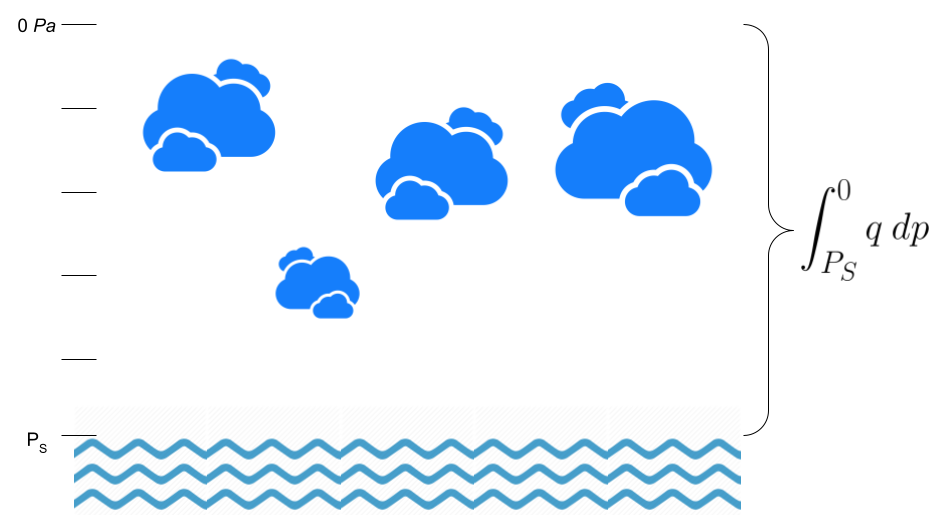
\includegraphics[width=\columnwidth]{imglib/water_vapor_integration.png}
    \end{figure}
    \end{column}
    
  \end{columns}
\end{frame}

\begin{frame}{Integrated Water Vapor Transport}

 \begin{columns}
   \begin{column}{0.55\textwidth}
Proposed by \citeauthor{zhu_proposed_1998}, 1998 \cite{zhu_proposed_1998}:\\
       $\bullet$ Goal: find \textbf{atmospheric rivers} 



    $$ 
    Q' = \ihat \frac{1}{g} \displaystyle\int_{P_0}^{300 hPa} \overline{q'u'} dp + \jhat \frac{1}{g} \displaystyle\int_{P_0}^{300 hPa} \overline{q'v'} dp
    $$
Since then in most cases: $||IVT||_2$ $\to$ Scalar field \cite{sousa_north_2020, jiang_impact_2017, ayantobo_integrated_2022, allan_diagnosing_2016, ralph_scale_2019, ralph_dropsonde_2017}
   \end{column}
   \begin{column}{0.45\textwidth}
    \begin{figure}[h]
      \centering
      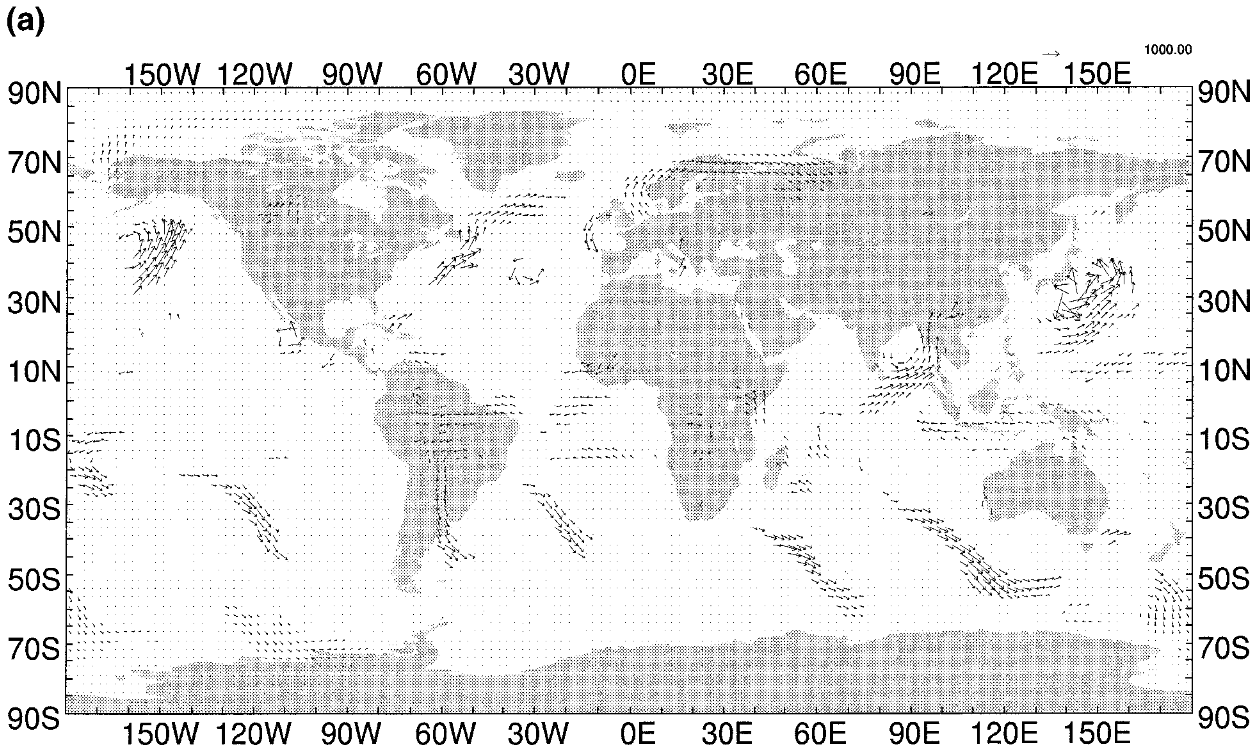
\includegraphics[width=\columnwidth]{imglib/zhu_ars.png}
    \end{figure}
    
   \end{column}
  
 \end{columns} 
  
  
\end{frame}

